\documentclass[11pt]{article}
\usepackage{tikz}
\usepackage{pgffor}
\usetikzlibrary{shapes}
\usetikzlibrary{arrows}
\usetikzlibrary{trees}
\usetikzlibrary{patterns}

\begin{document}

\begin{figure}
\begin{center}

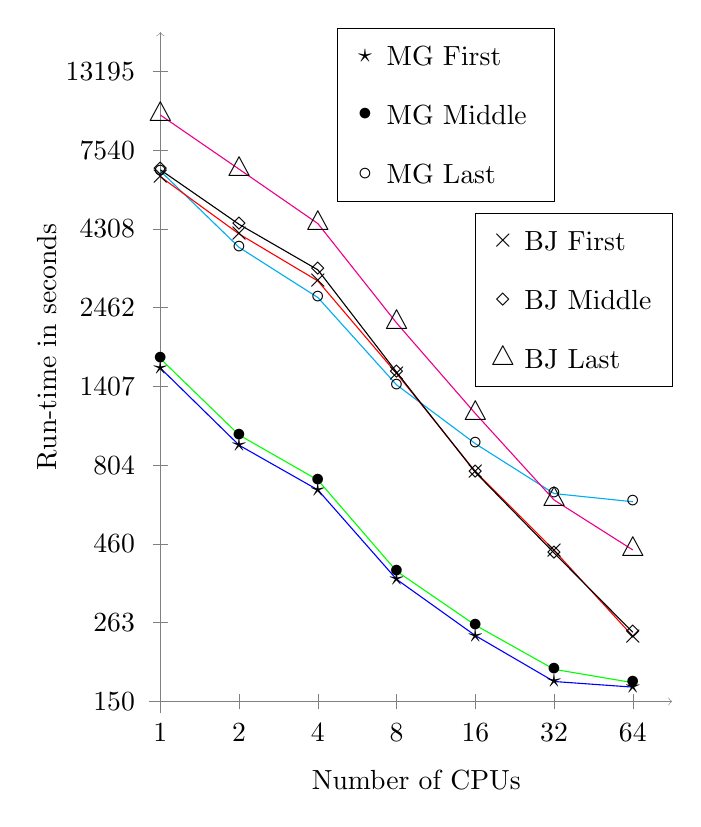
\begin{tikzpicture}[scale=1.0]

\draw[very thin, color=gray, ->] (-0.15, 0) -- (6.5, 0);
\draw[very thin, color=gray, ->] (0, -0.15) -- (0, 8.5);

\draw (3.25, -1) node {{Number of CPUs}};
\draw[color=white] (-1.2, 4) -- +(90:1) node[midway,sloped,above, color=black]{{Run-time in seconds}};

%Draw Row Ticks
\foreach \pos/\val in {0/1, 1/2, 2/4, 3/8, 4/16, 5/32, 6/64} {
\draw[very thin, color=gray] (\pos, -0.1) -- (\pos, 0.1);
\draw (\pos, -0.4) node {{\val}};
}

%Draw Col Ticks
\foreach \pos/\val in {0/150, 1/263, 2/460, 3/804, 4/1407, 5/2462, 6/4308, 7/7540, 8/13195} {
\draw[very thin, color=gray] (-0.1, \pos) -- (0.1, \pos);
\draw (-0.2, \pos) node[left] {{\val}};
}

%Draw legend

\path (-1, 1.75) coordinate (offb);

\draw (offb) ++ (3.25, 4.6) rectangle ++ (2.75, 2.2);
\draw (offb) ++ (3.75, 4.95) node[right] {MG Last};
\draw (offb) ++ (3.75, 5.7) node[right] {MG Middle};
\draw (offb) ++ (3.75, 6.45) node[right] {MG First};

\draw (offb) ++ (3.6, 4.95) node {$\circ$};
\draw (offb) ++ (3.6, 5.7) node {$\bullet$};
\draw (offb) ++ (3.6, 6.45) node {$\star$};

\path (0.75, -0.6) coordinate (offa);

\draw (offa) ++ (3.25, 4.6) rectangle ++ (2.5, 2.2);
\draw (offa) ++ (3.75, 4.95) node[right] {BJ Last};
\draw (offa) ++ (3.75, 5.7) node[right] {BJ Middle};
\draw (offa) ++ (3.75, 6.45) node[right] {BJ First};

\draw (offa) ++ (3.6, 4.95) node {$\triangle$};
\draw (offa) ++ (3.6, 5.7) node {$\diamond$};
\draw (offa) ++ (3.6, 6.45) node {$\times$};


 \draw[blue] 
  (0.000000, 4.234036) -- 
 (1.000000, 3.254105) -- 
 (2.000000, 2.686743) -- 
 (3.000000, 1.550958) -- 
 (4.000000, 0.836515) -- 
 (5.000000, 0.253368) -- 
 (6.000000, 0.182079) ; 
 
 
 \draw  (0.000000, 4.234036) node {$\star$}; 
 \draw  (1.000000, 3.254105) node {$\star$}; 
 \draw  (2.000000, 2.686743) node {$\star$}; 
 \draw  (3.000000, 1.550958) node {$\star$}; 
 \draw  (4.000000, 0.836515) node {$\star$}; 
 \draw  (5.000000, 0.253368) node {$\star$}; 
 \draw  (6.000000, 0.182079) node {$\star$}; 


 \draw[green] 
  (0.000000, 4.353210) -- 
 (1.000000, 3.383649) -- 
 (2.000000, 2.812355) -- 
 (3.000000, 1.654807) -- 
 (4.000000, 0.968824) -- 
 (5.000000, 0.408344) -- 
 (6.000000, 0.238732) ; 
 
 
 \draw  (0.000000, 4.353210) node {$\bullet$}; 
 \draw  (1.000000, 3.383649) node {$\bullet$}; 
 \draw  (2.000000, 2.812355) node {$\bullet$}; 
 \draw  (3.000000, 1.654807) node {$\bullet$}; 
 \draw  (4.000000, 0.968824) node {$\bullet$}; 
 \draw  (5.000000, 0.408344) node {$\bullet$}; 
 \draw  (6.000000, 0.238732) node {$\bullet$}; 


 \draw[cyan] 
  (0.000000, 6.736213) -- 
 (1.000000, 5.766367) -- 
 (2.000000, 5.130036) -- 
 (3.000000, 4.020163) -- 
 (4.000000, 3.273760) -- 
 (5.000000, 2.640132) -- 
 (6.000000, 2.536165) ; 
 
 
 \draw  (0.000000, 6.736213) node {$\circ$}; 
 \draw  (1.000000, 5.766367) node {$\circ$}; 
 \draw  (2.000000, 5.130036) node {$\circ$}; 
 \draw  (3.000000, 4.020163) node {$\circ$}; 
 \draw  (4.000000, 3.273760) node {$\circ$}; 
 \draw  (5.000000, 2.640132) node {$\circ$}; 
 \draw  (6.000000, 2.536165) node {$\circ$}; 



 \draw[red] 
  (0.000000, 6.664496) -- 
 (1.000000, 5.936620) -- 
 (2.000000, 5.340222) -- 
 (3.000000, 4.165087) -- 
 (4.000000, 2.920001) -- 
 (5.000000, 1.919623) -- 
 (6.000000, 0.828290) ; 
 
 
 \draw  (0.000000, 6.664496) node {$\times$}; 
 \draw  (1.000000, 5.936620) node {$\times$}; 
 \draw  (2.000000, 5.340222) node {$\times$}; 
 \draw  (3.000000, 4.165087) node {$\times$}; 
 \draw  (4.000000, 2.920001) node {$\times$}; 
 \draw  (5.000000, 1.919623) node {$\times$}; 
 \draw  (6.000000, 0.828290) node {$\times$}; 


 \draw[black] 
  (0.000000, 6.751721) -- 
 (1.000000, 6.059216) -- 
 (2.000000, 5.481430) -- 
 (3.000000, 4.181572) -- 
 (4.000000, 2.909813) -- 
 (5.000000, 1.886150) -- 
 (6.000000, 0.878682) ; 
 
 
 \draw  (0.000000, 6.751721) node {$\diamond$}; 
 \draw  (1.000000, 6.059216) node {$\diamond$}; 
 \draw  (2.000000, 5.481430) node {$\diamond$}; 
 \draw  (3.000000, 4.181572) node {$\diamond$}; 
 \draw  (4.000000, 2.909813) node {$\diamond$}; 
 \draw  (5.000000, 1.886150) node {$\diamond$}; 
 \draw  (6.000000, 0.878682) node {$\diamond$}; 


 \draw[magenta] 
  (0.000000, 7.447299) -- 
 (1.000000, 6.759520) -- 
 (2.000000, 6.069099) -- 
 (3.000000, 4.806343) -- 
 (4.000000, 3.656798) -- 
 (5.000000, 2.558586) -- 
 (6.000000, 1.924093) ; 
 
 
 \draw  (0.000000, 7.447299) node {$\triangle$}; 
 \draw  (1.000000, 6.759520) node {$\triangle$}; 
 \draw  (2.000000, 6.069099) node {$\triangle$}; 
 \draw  (3.000000, 4.806343) node {$\triangle$}; 
 \draw  (4.000000, 3.656798) node {$\triangle$}; 
 \draw  (5.000000, 2.558586) node {$\triangle$}; 
 \draw  (6.000000, 1.924093) node {$\triangle$}; 


\end{tikzpicture} 

\end{center}
\end{figure}

\end{document}
			